
%% bare_conf.tex
%% V1.3
%% 2007/01/11
%% by Michael Shell
%% See:
%% http://www.michaelshell.org/
%% for current contact information.
%%
%% This is a skeleton file demonstrating the use of IEEEtran.cls
%% (requires IEEEtran.cls version 1.7 or later) with an IEEE conference paper.
%%
%% Support sites:
%% http://www.michaelshell.org/tex/ieeetran/
%% http://www.ctan.org/tex-archive/macros/latex/contrib/IEEEtran/
%% and
%% http://www.ieee.org/

%%*************************************************************************
%% Legal Notice:
%% This code is offered as-is without any warranty either expressed or
%% implied; without even the implied warranty of MERCHANTABILITY or
%% FITNESS FOR A PARTICULAR PURPOSE! 
%% User assumes all risk.
%% In no event shall IEEE or any contributor to this code be liable for
%% any damages or losses, including, but not limited to, incidental,
%% consequential, or any other damages, resulting from the use or misuse
%% of any information contained here.
%%
%% All comments are the opinions of their respective authors and are not
%% necessarily endorsed by the IEEE.
%%
%% This work is distributed under the LaTeX Project Public License (LPPL)
%% ( http://www.latex-project.org/ ) version 1.3, and may be freely used,
%% distributed and modified. A copy of the LPPL, version 1.3, is included
%% in the base LaTeX documentation of all distributions of LaTeX released
%% 2003/12/01 or later.
%% Retain all contribution notices and credits.
%% ** Modified files should be clearly indicated as such, including  **
%% ** renaming them and changing author support contact information. **
%%
%% File list of work: IEEEtran.cls, IEEEtran_HOWTO.pdf, bare_adv.tex,
%%                    bare_conf.tex, bare_jrnl.tex, bare_jrnl_compsoc.tex
%%*************************************************************************

% *** Authors should verify (and, if needed, correct) their LaTeX system  ***
% *** with the testflow diagnostic prior to trusting their LaTeX platform ***
% *** with production work. IEEE's font choices can trigger bugs that do  ***
% *** not appear when using other class files.                            ***
% The testflow support page is at:
% http://www.michaelshell.org/tex/testflow/



% Note that the a4paper option is mainly intended so that authors in
% countries using A4 can easily print to A4 and see how their papers will
% look in print - the typesetting of the document will not typically be
% affected with changes in paper size (but the bottom and side margins will).
% Use the testflow package mentioned above to verify correct handling of
% both paper sizes by the user's LaTeX system.
%
% Also note that the "draftcls" or "draftclsnofoot", not "draft", option
% should be used if it is desired that the figures are to be displayed in
% draft mode.
%
\documentclass[10pt, conference, compsocconf]{IEEEtran}

% Add the compsocconf option for Computer Society conferences.
%
% If IEEEtran.cls has not been installed into the LaTeX system files,
% manually specify the path to it like:
% \documentclass[conference]{../sty/IEEEtran}





% Some very useful LaTeX packages include:
% (uncomment the ones you want to load)


% *** MISC UTILITY PACKAGES ***
%
\usepackage{ifpdf}
% Heiko Oberdiek's ifpdf.sty is very useful if you need conditional
% compilation based on whether the output is pdf or dvi.
% usage:
% \ifpdf
%   % pdf code
% \else
%   % dvi code
% \fi
% The latest version of ifpdf.sty can be obtained from:
% http://www.ctan.org/tex-archive/macros/latex/contrib/oberdiek/
% Also, note that IEEEtran.cls V1.7 and later provides a builtin
% \ifCLASSINFOpdf conditional that works the same way.
% When switching from latex to pdflatex and vice-versa, the compiler may
% have to be run twice to clear warning/error messages.






% *** CITATION PACKAGES ***
%
\usepackage{cite}
% cite.sty was written by Donald Arseneau
% V1.6 and later of IEEEtran pre-defines the format of the cite.sty package
% \cite{} output to follow that of IEEE. Loading the cite package will
% result in citation numbers being automatically sorted and properly
% "compressed/ranged". e.g., [1], [9], [2], [7], [5], [6] without using
% cite.sty will become [1], [2], [5]--[7], [9] using cite.sty. cite.sty's
% \cite will automatically add leading space, if needed. Use cite.sty's
% noadjust option (cite.sty V3.8 and later) if you want to turn this off.
% cite.sty is already installed on most LaTeX systems. Be sure and use
% version 4.0 (2003-05-27) and later if using hyperref.sty. cite.sty does
% not currently provide for hyperlinked citations.
% The latest version can be obtained at:
% http://www.ctan.org/tex-archive/macros/latex/contrib/cite/
% The documentation is contained in the cite.sty file itself.






% *** GRAPHICS RELATED PACKAGES ***
%
\ifCLASSINFOpdf
   \usepackage[pdftex]{graphicx}
%   \usepackage{subfigure}
  % declare the path(s) where your graphic files are
  % \graphicspath{{../pdf/}{../jpeg/}}
  % and their extensions so you won't have to specify these with
  % every instance of \includegraphics
  % \DeclareGraphicsExtensions{.pdf,.jpeg,.png}
\else
  % or other class option (dvipsone, dvipdf, if not using dvips). graphicx
  % will default to the driver specified in the system graphics.cfg if no
  % driver is specified.
   \usepackage[dvips]{graphicx}
  % declare the path(s) where your graphic files are
  % \graphicspath{{../eps/}}
  % and their extensions so you won't have to specify these with
  % every instance of \includegraphics
  % \DeclareGraphicsExtensions{.eps}
\fi
% graphicx was written by David Carlisle and Sebastian Rahtz. It is
% required if you want graphics, photos, etc. graphicx.sty is already
% installed on most LaTeX systems. The latest version and documentation can
% be obtained at: 
% http://www.ctan.org/tex-archive/macros/latex/required/graphics/
% Another good source of documentation is "Using Imported Graphics in
% LaTeX2e" by Keith Reckdahl which can be found as epslatex.ps or
% epslatex.pdf at: http://www.ctan.org/tex-archive/info/
%
% latex, and pdflatex in dvi mode, support graphics in encapsulated
% postscript (.eps) format. pdflatex in pdf mode supports graphics
% in .pdf, .jpeg, .png and .mps (metapost) formats. Users should ensure
% that all non-photo figures use a vector format (.eps, .pdf, .mps) and
% not a bitmapped formats (.jpeg, .png). IEEE frowns on bitmapped formats
% which can result in "jaggedy"/blurry rendering of lines and letters as
% well as large increases in file sizes.
%
% You can find documentation about the pdfTeX application at:
% http://www.tug.org/applications/pdftex





% *** MATH PACKAGES ***
%
\usepackage[cmex10]{amsmath}
% A popular package from the American Mathematical Society that provides
% many useful and powerful commands for dealing with mathematics. If using
% it, be sure to load this package with the cmex10 option to ensure that
% only type 1 fonts will utilized at all point sizes. Without this option,
% it is possible that some math symbols, particularly those within
% footnotes, will be rendered in bitmap form which will result in a
% document that can not be IEEE Xplore compliant!
%
% Also, note that the amsmath package sets \interdisplaylinepenalty to 10000
% thus preventing page breaks from occurring within multiline equations. Use:
%\interdisplaylinepenalty=2500
% after loading amsmath to restore such page breaks as IEEEtran.cls normally
% does. amsmath.sty is already installed on most LaTeX systems. The latest
% version and documentation can be obtained at:
% http://www.ctan.org/tex-archive/macros/latex/required/amslatex/math/





% *** SPECIALIZED LIST PACKAGES ***
%
\usepackage{algorithmic}
% algorithmic.sty was written by Peter Williams and Rogerio Brito.
% This package provides an algorithmic environment fo describing algorithms.
% You can use the algorithmic environment in-text or within a figure
% environment to provide for a floating algorithm. Do NOT use the algorithm
% floating environment provided by algorithm.sty (by the same authors) or
% algorithm2e.sty (by Christophe Fiorio) as IEEE does not use dedicated
% algorithm float types and packages that provide these will not provide
% correct IEEE style captions. The latest version and documentation of
% algorithmic.sty can be obtained at:
% http://www.ctan.org/tex-archive/macros/latex/contrib/algorithms/
% There is also a support site at:
% http://algorithms.berlios.de/index.html
% Also of interest may be the (relatively newer and more customizable)
% algorithmicx.sty package by Szasz Janos:
% http://www.ctan.org/tex-archive/macros/latex/contrib/algorithmicx/




% *** ALIGNMENT PACKAGES ***
%
\usepackage{array}
% Frank Mittelbach's and David Carlisle's array.sty patches and improves
% the standard LaTeX2e array and tabular environments to provide better
% appearance and additional user controls. As the default LaTeX2e table
% generation code is lacking to the point of almost being broken with
% respect to the quality of the end results, all users are strongly
% advised to use an enhanced (at the very least that provided by array.sty)
% set of table tools. array.sty is already installed on most systems. The
% latest version and documentation can be obtained at:
% http://www.ctan.org/tex-archive/macros/latex/required/tools/


\usepackage{mdwmath}
\usepackage{mdwtab}
% Also highly recommended is Mark Wooding's extremely powerful MDW tools,
% especially mdwmath.sty and mdwtab.sty which are used to format equations
% and tables, respectively. The MDWtools set is already installed on most
% LaTeX systems. The lastest version and documentation is available at:
% http://www.ctan.org/tex-archive/macros/latex/contrib/mdwtools/


% IEEEtran contains the IEEEeqnarray family of commands that can be used to
% generate multiline equations as well as matrices, tables, etc., of high
% quality.


\usepackage{eqparbox}
% Also of notable interest is Scott Pakin's eqparbox package for creating
% (automatically sized) equal width boxes - aka "natural width parboxes".
% Available at:
% http://www.ctan.org/tex-archive/macros/latex/contrib/eqparbox/





% *** SUBFIGURE PACKAGES ***
\usepackage[tight,footnotesize]{subfigure}
% subfigure.sty was written by Steven Douglas Cochran. This package makes it
% easy to put subfigures in your figures. e.g., "Figure 1a and 1b". For IEEE
% work, it is a good idea to load it with the tight package option to reduce
% the amount of white space around the subfigures. subfigure.sty is already
% installed on most LaTeX systems. The latest version and documentation can
% be obtained at:
% http://www.ctan.org/tex-archive/obsolete/macros/latex/contrib/subfigure/
% subfigure.sty has been superceeded by subfig.sty.



%\usepackage[caption=false]{caption}
%\usepackage[font=footnotesize]{subfig}
% subfig.sty, also written by Steven Douglas Cochran, is the modern
% replacement for subfigure.sty. However, subfig.sty requires and
% automatically loads Axel Sommerfeldt's caption.sty which will override
% IEEEtran.cls handling of captions and this will result in nonIEEE style
% figure/table captions. To prevent this problem, be sure and preload
% caption.sty with its "caption=false" package option. This is will preserve
% IEEEtran.cls handing of captions. Version 1.3 (2005/06/28) and later 
% (recommended due to many improvements over 1.2) of subfig.sty supports
% the caption=false option directly:
%\usepackage[caption=false,font=footnotesize]{subfig}
%
% The latest version and documentation can be obtained at:
% http://www.ctan.org/tex-archive/macros/latex/contrib/subfig/
% The latest version and documentation of caption.sty can be obtained at:
% http://www.ctan.org/tex-archive/macros/latex/contrib/caption/




% *** FLOAT PACKAGES ***
%
\usepackage{fixltx2e}
% fixltx2e, the successor to the earlier fix2col.sty, was written by
% Frank Mittelbach and David Carlisle. This package corrects a few problems
% in the LaTeX2e kernel, the most notable of which is that in current
% LaTeX2e releases, the ordering of single and double column floats is not
% guaranteed to be preserved. Thus, an unpatched LaTeX2e can allow a
% single column figure to be placed prior to an earlier double column
% figure. The latest version and documentation can be found at:
% http://www.ctan.org/tex-archive/macros/latex/base/



\usepackage{stfloats}
% stfloats.sty was written by Sigitas Tolusis. This package gives LaTeX2e
% the ability to do double column floats at the bottom of the page as well
% as the top. (e.g., "\begin{figure*}[!b]" is not normally possible in
% LaTeX2e). It also provides a command:
%\fnbelowfloat
% to enable the placement of footnotes below bottom floats (the standard
% LaTeX2e kernel puts them above bottom floats). This is an invasive package
% which rewrites many portions of the LaTeX2e float routines. It may not work
% with other packages that modify the LaTeX2e float routines. The latest
% version and documentation can be obtained at:
% http://www.ctan.org/tex-archive/macros/latex/contrib/sttools/
% Documentation is contained in the stfloats.sty comments as well as in the
% presfull.pdf file. Do not use the stfloats baselinefloat ability as IEEE
% does not allow \baselineskip to stretch. Authors submitting work to the
% IEEE should note that IEEE rarely uses double column equations and
% that authors should try to avoid such use. Do not be tempted to use the
% cuted.sty or midfloat.sty packages (also by Sigitas Tolusis) as IEEE does
% not format its papers in such ways.





% *** PDF, URL AND HYPERLINK PACKAGES ***
%
\usepackage{url}
% url.sty was written by Donald Arseneau. It provides better support for
% handling and breaking URLs. url.sty is already installed on most LaTeX
% systems. The latest version can be obtained at:
% http://www.ctan.org/tex-archive/macros/latex/contrib/misc/
% Read the url.sty source comments for usage information. Basically,
% \url{my_url_here}.


\usepackage{booktabs}



% *** Do not adjust lengths that control margins, column widths, etc. ***
% *** Do not use packages that alter fonts (such as pslatex).         ***
% There should be no need to do such things with IEEEtran.cls V1.6 and later.
% (Unless specifically asked to do so by the journal or conference you plan
% to submit to, of course. )


% correct bad hyphenation here
\hyphenation{op-tical net-works semi-conduc-tor}
\DeclareRobustCommand*{\IEEEauthorrefmark}[1]{%
	\raisebox{0pt}[0pt][0pt]{\textsuperscript{\footnotesize\ensuremath{#1}}}}{\tiny }

\begin{document}
%
% paper title
% can use linebreaks \\ within to get better formatting as desired
\title{Improve Accuracy of Speech Emotion Recognition with Attention Head Fusion}


% author names and affiliations
% use a multiple column layout for up to two different
% affiliations

\author{
	\IEEEauthorblockN{Mingke Xu}
	\IEEEauthorblockA{Computer Science and Technology \\
		Nanjing Tech University \\
		Jiangsu Province, China \\
		201861120004@njtech.edu.cn}
	\and
	\IEEEauthorblockN{Fan Zhang}
	\IEEEauthorblockA{IBM Watson Group \\
		IBM Massachusette Lab \\
		Littleton, MA\\
		fzhang@us.ibm.com}
}

% conference papers do not typically use \thanks and this command
% is locked out in conference mode. If really needed, such as for
% the acknowledgment of grants, issue a \IEEEoverridecommandlockouts
% after \documentclass

% for over three affiliations, or if they all won't fit within the width
% of the page, use this alternative format:
% 
%\author{\IEEEauthorblockN{Michael Shell\IEEEauthorrefmark{1},
%Homer Simpson\IEEEauthorrefmark{2},
%James Kirk\IEEEauthorrefmark{3}, 
%Montgomery Scott\IEEEauthorrefmark{3} and
%Eldon Tyrell\IEEEauthorrefmark{4}}
%\IEEEauthorblockA{\IEEEauthorrefmark{1}School of Electrical and Computer Engineering\\
%Georgia Institute of Technology,
%Atlanta, Georgia 30332--0250\\ Email: see http://www.michaelshell.org/contact.html}
%\IEEEauthorblockA{\IEEEauthorrefmark{2}Twentieth Century Fox, Springfield, USA\\
%Email: homer@thesimpsons.com}
%\IEEEauthorblockA{\IEEEauthorrefmark{3}Starfleet Academy, San Francisco, California 96678-2391\\
%Telephone: (800) 555--1212, Fax: (888) 555--1212}
%\IEEEauthorblockA{\IEEEauthorrefmark{4}Tyrell Inc., 123 Replicant Street, Los Angeles, California 90210--4321}}




% use for special paper notices
%\IEEEspecialpapernotice{(Invited Paper)}




% make the title area
\maketitle


\begin{abstract}
%The abstract goes here. DO NOT USE SPECIAL CHARACTERS, SYMBOLS, OR MATH IN YOUR %TITLE OR ABSTRACT.
Speech Emotion Recognition (SER) refers to the use of machines to recognize the emotions of a speaker from his (or her) speech. In this paper, we propose a multi-head self-attention based attention method to improve the recognition accuracy of SER. We call this method head fusion. We combined this method to implement an ACNN model, using MFCCs extracted from speech and conducted experiments and evaluations on the IEMOCAP dataset. 76.18\% of WA and 76.36\% of UA were obtained on the improvised part, both better than state-of-the-art.
\end{abstract}

\begin{IEEEkeywords}
%component; formatting; style; styling;
speech emotion recognition; convolutional neural network; self-attention
\end{IEEEkeywords}


% For peer review papers, you can put extra information on the cover
% page as needed:
% \ifCLASSOPTIONpeerreview
% \begin{center} \bfseries EDICS Category: 3-BBND \end{center}
% \fi
%
% For peerreview papers, this IEEEtran command inserts a page break and
% creates the second title. It will be ignored for other modes.
\IEEEpeerreviewmaketitle



\section{Introduction}
% no \IEEEPARstart
%This demo file is intended to serve as a ``starter file''
%for IEEE conference papers produced under \LaTeX\ using
%IEEEtran.cls version 1.7 and later.
%
%All manuscripts must be in English. These guidelines include complete descriptions of the fonts, spacing, and related information for producing your proceedings manuscripts. Please follow them and if you have any questions, direct them to the production editor in charge of your proceedings at Conference Publishing Services (CPS): Phone +1 (714) 821-8380 or Fax +1 (714) 761-1784.
Today, machine speech recognition services such as Auto Speech Recognition (ASR) have been widely used in society. The machine can easily recognize what humans are talking about. Speech Emotion Recognition (SER) also has broad prospects in the field of criminal investigation, medical care, etc. However, for machines, it is still a huge challenge to recognize emotional content in human discourse.

Unlike general ASR, since emotions are subjective and influenced by many factors, how to obtain accurate and recognized high-quality labeled emotional speech data is important in SER. According to R. Altrov \emph{et al.} \cite{altrov2015influence}, language and culture have an important influence on the judgment of emotions in speech. Fortunately, the IEMOCAP corpus established by C. Busso \emph{et al.} effectively solved the problem of lack of data in SER \cite{busso2008iemocap}. This corpus has been frequently used in the field of SER.

However, the current SER model still does not accurately recognize human emotions. On the IEMOCAP corpus, the state of the art recognition accuracy is 70.17\% for weighted accuracy(WA), and 70.85\% for unweighted accuracy (UA)\cite{tarantino2019self}. We believe that there is still much room for improvement in this accuracy.
In this paper, we propose an approach based on multi-head self-attention and architecture combined with attention mechanism and Convolutional Neural Network (CNN) for SER. It achieved state of the art recognition accuracy on IEMOCAP.

In this paper, our main contributions are as follows:

1) We proposed a method based on multi-head self-attention. We call this method head fusion. Using this method increases the recognition accuracy by about 6\% in the IEMOCAP corpus compared to the normal self-attention structure.
2) We implemented an SER model combining CNN and attention and performed experiments on the IEMOCAP corpus, reaching 76.18\% of WA and 76.36\% of UA, which is state of the art.

% You must have at least 2 lines in the paragraph with the drop letter
% (should never be an issue)

%\subsection{Subsection Heading Here}
%Subsection text here.
%
%
%\subsubsection{Subsubsection Heading Here}
%Subsubsection text here.

%\section{Type style and Fonts}
%Wherever Times is specified, Times Roman or Times New Roman may be used. If neither is available on your system, please use the font closest in appearance to Times. Avoid using bit-mapped fonts if possible. True-Type 1 or Open Type fonts are preferred. Please embed symbol fonts, as well, for math, etc.

\section{RELATED WORK}
Before the era of deep learning, for SER, researchers mostly use complex hand-crafted features (such as IS09, eGeMaps, etc.) and traditional machine learning methods (such as HMM, SVM, etc.) \cite{schuller2003hidden,mower2010framework}. In 2014, K. Han \emph{et al.} proposed the first end-to-end deep learning SER model \cite{han2014speech}. Later, with the development of deep learning technology, more and more deep learning models for SER were proposed.

Vladimir Chernykh \emph{et al.} proposed a CTC-based RNN network that uses hand-crafted 34-dimensional features for emotional classification \cite{chernykh2017emotion}. Abdul Malik Badshah \emph{et al.} inputted the spectrogram as features into deep CNN for classification \cite{badshah2017speech}. Xixin Wu \emph{et al.} used the spectrogram and replaced the traditional convolution network with CapsNet, which achieved better classification results \cite{wu2019speech}. 

At present, the attention mechanism is being used more and more in the field of deep learning, especially after Google has greatly improved the accuracy of machine translation \cite{vaswani2017attention}. In the field of speech recognition, attention mechanism has been used in many tasks such as ASR \cite{pham2019very}, speaker recognition \cite{india2019self} and SER \cite{li2018attention,tarantino2019self,zhao2019attention,chen20183}.

Pengcheng Li \emph{et al.} proposed a mechanism called attention pooling that uses a spectrogram as input to apply top-down and bottom-up attention \cite{li2018attention}. Lorenzo Tarantino \emph{et al.} uses a combination of general self-attention and CNN, using a hand-crafted feature set \cite{tarantino2019self}. Ziping Zhao \emph{et al.} combines the Connectionist Temporal Classification(CTC) method and attention mechanism to convert classification problems into transfer problems by adding silent labels \cite{zhao2019attention}. Mingyi Chen \emph{et al.} uses the mel-spectrum, its delta and its second-order delta as inputs, combines CNN and RNN, and uses an attention layer at the end \cite{chen20183}.

In addition, some studies combine speech and text for recognition. For example, Seunghyun Yoon \emph{et al.} use ASR to obtain text, use an attention mechanism to calculate speech-related parts from the text, and use BLSTM for recognition \cite{yoon2019speech}.

\section{MODEL ARCHITECTURE AND HEAD FUSION}
SER is a classification problem that extracting features from human speech and inputting them into traditional machine learning algorithms or deep neural networks for recognition. Emotions are subjective and complex. If the tendency of emotions (positive or negative) is the same, the differences between them are so small that even humans can not easily and accurately distinguish, which brings great difficulties to SER. In order to improve the accuracy of SER, we propose the following methods.
\subsection{Feature Extraction}
We use MFCCs as input, an audio feature that is widely used in the field of speech recognition. First, we use a Hanning window with a length of 2048 and a hop length of 512 to perform a short term Fourier transform (STFT) on the audio signal and obtain the power spectrum of the audio signal. Then we use mel filters to map the spectrum to Mel-scale and log to obtain the log Mel-spectrum. Finally, we use a DCT transformation to obtain 13 MFCCs.
\subsection{Model Architecture}
Figure \ref{model} shows the overall structure of our model, which consists mainly of a convolutional layer and an attention layer.
We use the extracted MFCCs as input and treat this input as an image, using two convolutional layers with a kernel size of (10,2) and (2,8) to extract the horizontal (cross-time) and vertical (cross-MFCC) textures, respectively. After padding, the 8-channel output of each convolutional layer is concatenated to a 16-channel representation. Then 4 convolution layers are applied to generate an 80-channel representation and sent to the self-attention layer. 
Table \ref{ConvSettings} shows the specific settings for the convolutional layers. After each convolutional layer, a Batch Normalization (BN) layer and an activation function Relu are used, and conv2 and conv3 are followed by max-pooling with a kernel size of 2 to reduce the data size.
\begin{table}[h]
	\renewcommand\arraystretch{1.5}
	\setlength{\abovecaptionskip}{-0.2cm}
	\caption{The specific settings for the convolutional layers.}
	\label{ConvSettings}
	\begin{center}  
		\begin{tabular}{|c|c|} 
			\hline  
			Name & Settings \\   
			\hline  
			Conv1a & kernel size=(10,2),stride=1,in channels=1,out channels=8\\   
			\hline
			Conv1b & kernel size=(2,8),stride=1,in channels=1,out channels=8 \\   
			\hline
			Conv2 & kernel size=(3,3),stride=1,in channels=16,out channels=32 \\   
			\hline
			Conv3 & kernel size=(3,3),stride=1,in channels=32,out channels=48 \\   
			\hline
			Conv4 & kernel size=(3,3),stride=1,in channels=48,out channels=64 \\   
			\hline
			Conv5 & kernel size=(3,3),stride=1,in channels=64,out channels=80 \\   
			\hline
		\end{tabular}  
	\end{center}  
\end{table}

\begin{figure}[h]
	\centering
	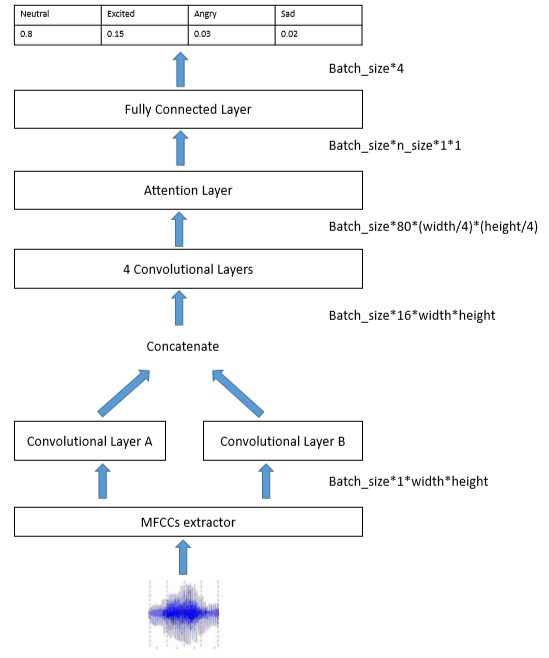
\includegraphics[width=0.95\linewidth]{pic/Model_Architecture}
	\caption{Overall structure of our ACNN model.}
	\label{model}
\end{figure}
\subsection{Self-Attention Layer and Head Fusion}
For the 80-channel representation X$_{cnn}$ generated by CNN, we calculate
\begin{equation}
\begin{split}
\displaystyle
K=W_k*X_{cnn},
Q=W_q*X_{cnn},
V=W_v*X_{cnn},
\end{split}
\end{equation}
where W$_k$, W$_q$, W$_v$ are trainable parameters.
After this we calculate
\begin{equation}
\begin{split}
\displaystyle
X_{attn}=Softmax(KQ^T)V
\end{split}
\end{equation}
to obtain X$_{attn}$——an attention map of X$_{cnn}$. We use X$_{attn}$$^i$ to represent i$_{th}$ X$_{attn}$ and calculate X$_{attn}$$^i$ by using different parameter sets W$_k$$^i$, W$_q$$^i$, W$_v$$^i$,where $i \in (0,n\_head]$, and each X$_{attn}$$^i$ is called a head. Different from the general self-attention, we superimpose heads to obtain an attention map with multiple points of attention.
\begin{equation}
\begin{split}
\displaystyle
X_{mattn}=\frac{\sum_{0}^{n\_head-1}X_{attn}^i}{n\_head}
\end{split}
\end{equation}

Then we use global average pooling (GAP) to generate a feature point X$_{fusion}$ for this map. In the past computer vision research, GAP has been proved to be an effective method \cite{he2016deep}. We call this superposition method head fusion. We set hyperparameter n\_head to represent how many heads being fused in a feature point and n\_size to represent how many feature points to generate. Finally, we concatenate these points and feed them to the fully connected layer to obtain the final classification result.
Figure \ref{headFusion} shows the working process of head fusion.

\begin{figure}[h]
	\centering
	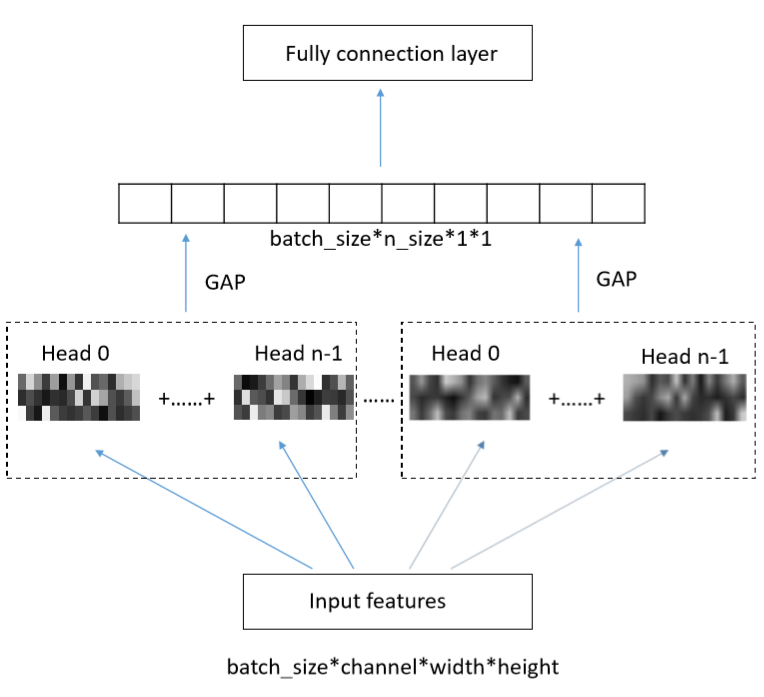
\includegraphics[width=0.95\linewidth]{pic/head_fusion}
	\caption{The working process of head fusion.}
	\label{headFusion}
\end{figure}

\section{EXPERIMENTAL EVALUATIONS}
\subsection{Data Set}
We use the IEMOCAP corpus as the experimental data set. It is widely used in SER and contains a total of about 12 hours of labeled emotional speech data. It consists of nine emotions: anger, happiness, excitement, sadness, frustration, fear, surprise, other and neutral state. Each utterance is evaluated by an evaluator of 3 or more people, and the utterance will be labeled with the corresponding emotion only if more than half of the evaluators agree, else, it will be labeled with 'other'. 

The IEMOCAP corpus is divided into two parts: scripted part and improvised part, that is, the actors perform according to the script and improvisation. In general, the accuracy of the classification of the improvised part is higher than that of the scripted part, because actors do not need to pay attention to the content of the words and express emotions more naturally \cite{li2018attention,tarantino2019self}.

Figure \ref{dataDistribution} shows the distribution of data in the IEMOCAP corpus.

\begin{figure}[h]
	
	\centering
	\subfigcapskip=5pt
	\subfigure[Distribution of utterances with 9 emotions.]{
		\begin{minipage}{8cm}
			\centering
			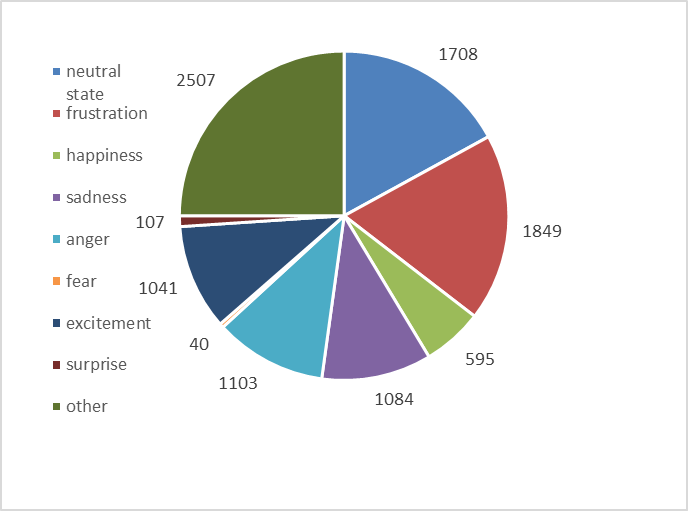
\includegraphics[width=0.85\columnwidth]{pic/emoInIEMOCAP}
	\end{minipage}}
	\subfigure[Distribution of utterances improvised or scripted.]{
		\begin{minipage}{8cm}
			\centering
			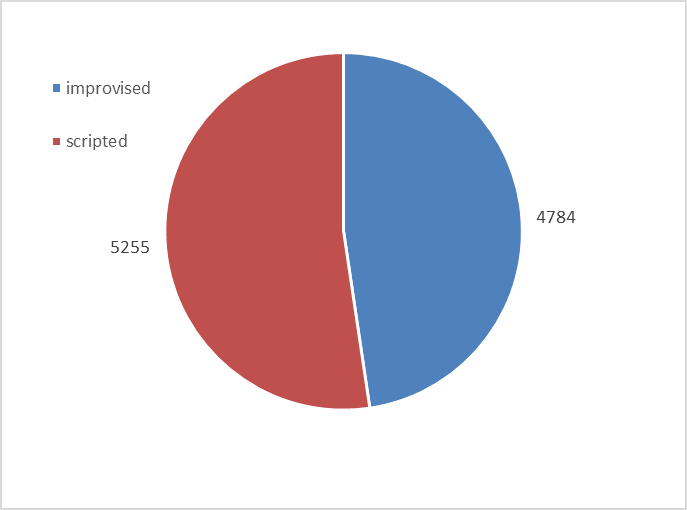
\includegraphics[width=0.85\columnwidth]{pic/ImproOrScript}
	\end{minipage}}
	\caption{Figure (a) shows the distribution of utterances with 9 emotions and Figure (b) shows the distribution of utterances improvised or scripted in the IEMOCAP corpus.}
	\label{dataDistribution}
	
\end{figure}
Since the happy class in IEMOCAP is too rare, researchers sometimes choose to use excitement class instead of happy class \cite{tarantino2019self,chernykh2017emotion} or merge samples from happy class and excitement class \cite{zhao2019attention,neumann2019improving}. We selected the improvised part of four emotions (angry, sad, excited and neutral) for our experiment to compare with previous research. Besides, we
tested our best model on the scripted part and full corpus to compare with the self-attention architecture in \cite{tarantino2019self}.

 

\subsection{Experimental Setup}
\subsubsection{Pre-treatment}
For each utterance, we segment it into segments of length 2 seconds and drop the parts that are too short. In the training set, in order to obtain more training data, there is an overlap of 1 second between each segment. These segments are given the label of their source utterance and participate in training as independent data. In the test set, segments from the same utterance are used together, and the results are averaged to obtain predictions. We set the overlap to 1.6 seconds to get better predictions.
Figure \ref{pre-treat} shows the 2 different ways to pre-treat data in the train set and the test set.

\begin{figure}[h]
	
	\centering
	\subfigcapskip=5pt
	\subfigure[The way of pre-treatment in train set.]{
	\begin{minipage}{10cm}
		\flushleft
%		\centering
		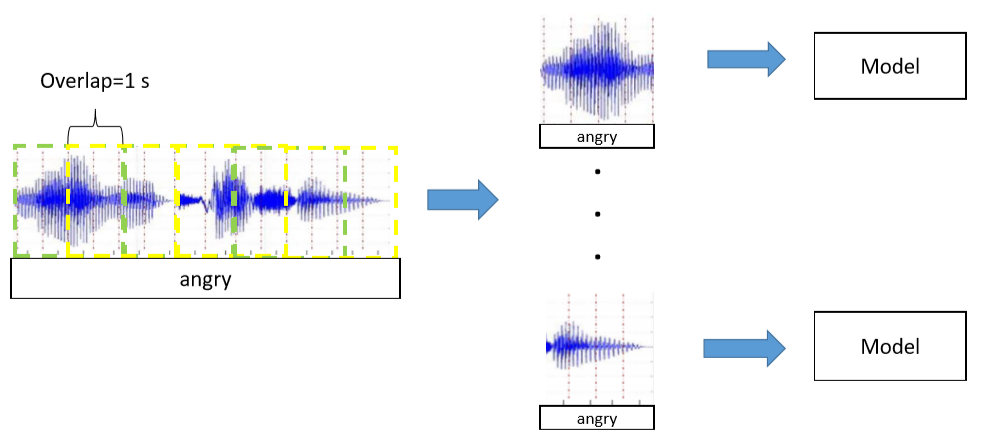
\includegraphics[width=0.85\columnwidth]{pic/train_set}
	\end{minipage}}
	\subfigure[The way of pre-treatment in test set.]{
		\begin{minipage}{10cm}
			\flushleft
%			\centering
			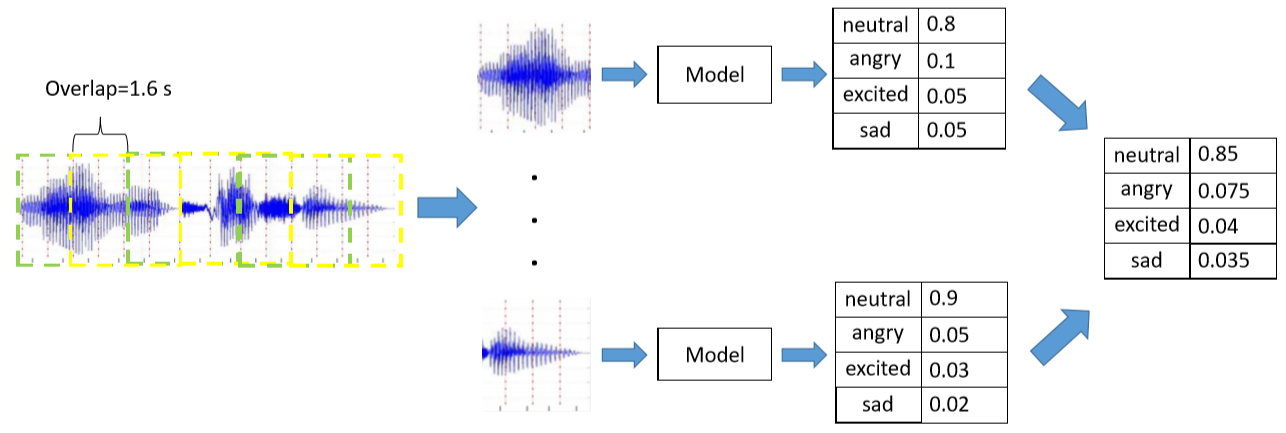
\includegraphics[width=0.85\columnwidth]{pic/test_set}
\end{minipage}}
	\caption{As shown in Figure (a), in the train set, we segment an utterance into segments of length 2 seconds with an overlap of length 1 second between each segment and use them as independent data in training. As shown in Figure (b), in the test set, we segment an utterance into segments of length 2 seconds with an overlap of length 1.6 seconds between each segment and average the prediction of each segment of a source utterance to obtain the final prediction.}
	\label{pre-treat}
	
\end{figure}

\subsubsection{Verification Method}
To compare with previous studies, we used 5-fold cross-validation, randomly selected 80\% data for training and 20\% data for testing. We implemented the model with PyTorch, used the cross-entropy loss function, and optimized it with the Adam optimizer. The batch size was set to 32. The initial learning rate was 0.001, weight decay was 1e-6, and the learning rate was manually set to 1/10 for every 10 epochs. We trained the model with 50 epochs on a GTX 1060 GPU and evaluated its WA and UA, saving the best model. For each parameter setting, we used 5 different random seeds for training and testing and averaged the accuracy to reduce the error.

\subsection{Results and Analysis}
In the experiment, the accuracy is improved compared to the self-attention model without head fusion, and the value of n\_head has a significant effect on the experimental results. We find that as n\_head increases, the accuracy increases gradually and reaches a maximum at a certain point. Then, if n\_head continues to increase, the accuracy will gradually decrease. We believe that the reason for this decline is that the value of n\_head is too high, causing some attention points in the map to be placed in too much detail, which will reduce the effect of attention instead.

Figure \ref{HeadResult} shows the change in accuracy caused by changing the value of n\_head when n\_size is set to 32, 64, and 128.
When n\_size is set to 32 or 64, we obtain the highest accuracy when n\_head is set to 4, and when n\_size is set to 128, we obtain the highest accuracy when n\_head is set to 3.We set n\_head to 4 in our final model.

\begin{figure}[h]
	
	\subfigcapskip=5pt
	\centering
	\subfigure[when n\_size is set to 32, we obtain the highest accuracy when n\_head is set to 4]{
		\begin{minipage}{8cm}
			\centering
%			\flushleft
			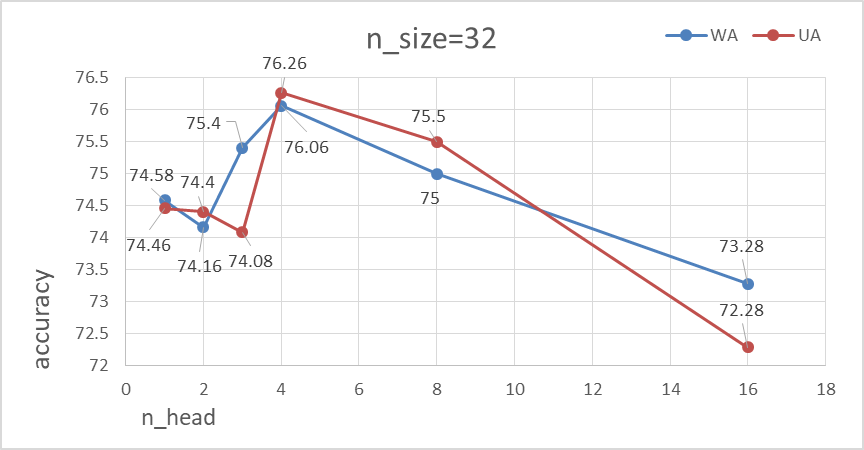
\includegraphics[width=0.93\linewidth]{pic/n_size32}
	\end{minipage}}
	\subfigure[when n\_size is set to 64, we obtain the highest accuracy when n\_head is set to 4]{
		\begin{minipage}{8cm}
			\centering
%			\flushleft
			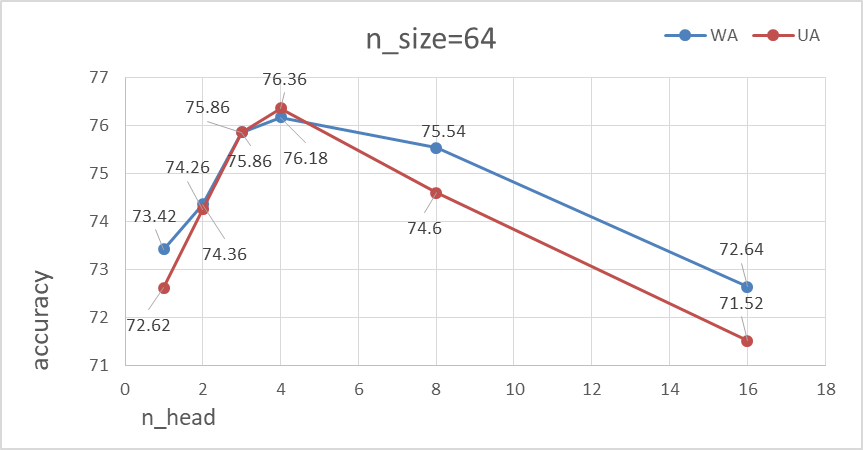
\includegraphics[width=0.93\linewidth]{pic/n_size64}
	\end{minipage}}
		\subfigure[when n\_size is set to 128, we obtain the highest accuracy when n\_head is set to 3]{
		\begin{minipage}{8cm}
			\centering
%			\flushleft
			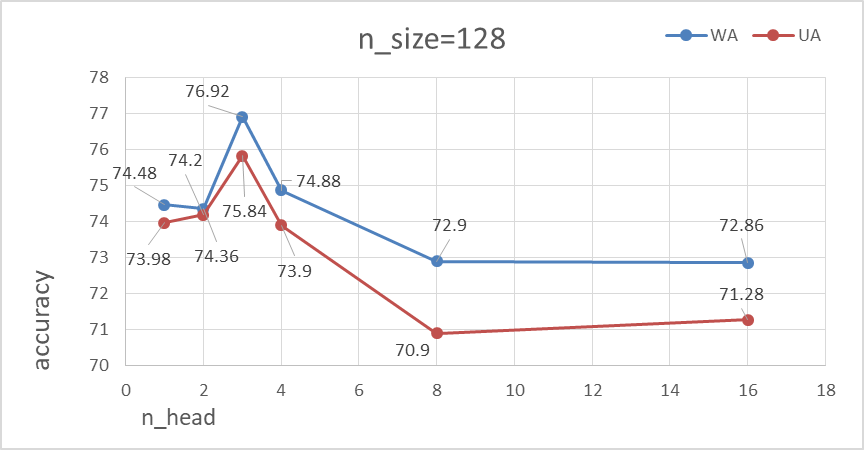
\includegraphics[width=0.93\linewidth]{pic/n_size128}
	\end{minipage}}
	\caption{Figure (a) shows the accuracy when n\_size is set to 32, Figure (b) shows the accuracy when n\_size is set to 64 and Figure (c) shows the accuracy when n\_size is set to 128. As shown, when n\_size is set to 32 or 64, we obtain the highest accuracy when n\_head is set to 4, and when n\_size is set to 128, we obtain the highest accuracy when n\_head is set to 3.}
	\label{HeadResult}
\end{figure}


As shown in Figure \ref{SizeResult}, we also tested the effect of different n\_sizes on accuracy with n\_head set to 2,4 and 8. When n\_head is set to 2, we obtain the highest accuracy when n\_size is set to 16, when n\_head is set to 4, we obtain the highest accuracy when n\_size is set to 64, and when n\_head is set to 8, we obtain the highest accuracy when n\_size is set to 32. We set n\_size to 64 in our final model.

\begin{figure}[h]
	
	\subfigcapskip=5pt
	\centering
	\subfigure[when n\_head is set to 2, we obtain the highest accuracy when n\_size is set to 16]{
		\begin{minipage}{8cm}
			\centering
%			\flushleft
			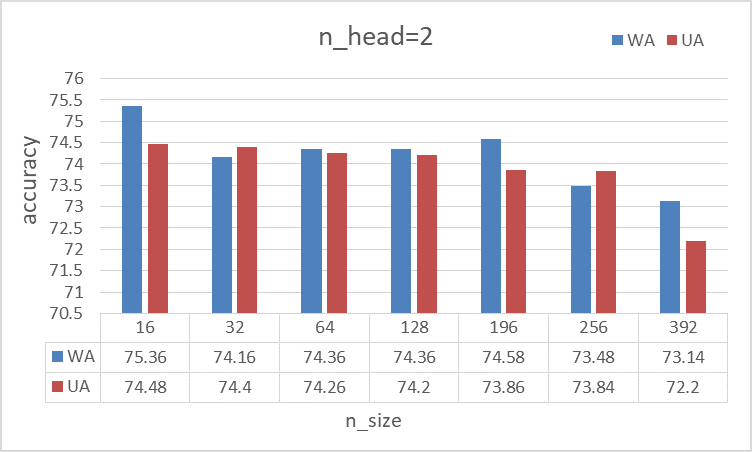
\includegraphics[width=0.93\linewidth]{pic/n_head2}
	\end{minipage}}
	\subfigure[when n\_head is set to 4, we obtain the highest accuracy when n\_size is set to 64]{
		\begin{minipage}{8cm}
			\centering
%			\flushleft
			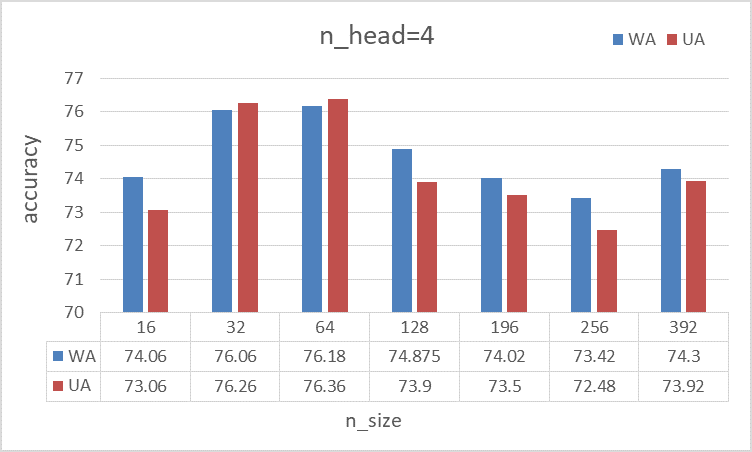
\includegraphics[width=0.93\linewidth]{pic/n_head4}
	\end{minipage}}
	\subfigure[when n\_head is set to 8, we obtain the highest accuracy when n\_size is set to 32]{
		\begin{minipage}{8cm}
			\centering
%			\flushleft
			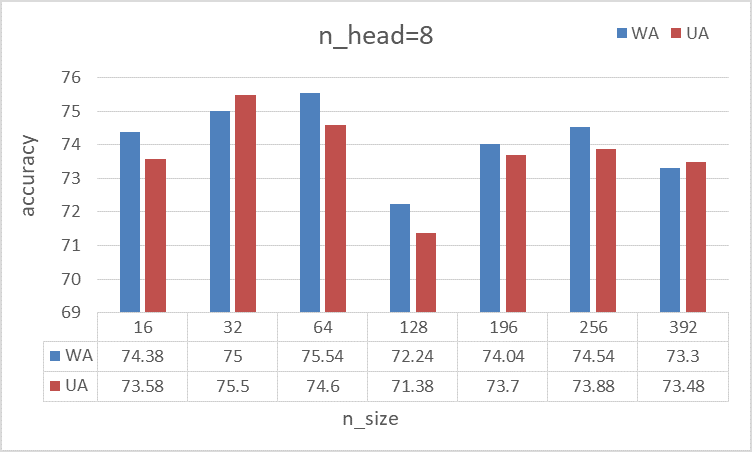
\includegraphics[width=0.93\linewidth]{pic/n_head8}
	\end{minipage}}
	\caption{Figure (a) shows the accuracy when n\_head is set to 2, Figure (b) shows the accuracy when n\_head is set to 4 and Figure (c) shows the accuracy when n\_head is set to 8. As shown, when n\_head is set to 2, we obtain the highest accuracy when n\_size is set to 16, when n\_head is set to 4, we obtain the highest accuracy when n\_size is set to 64, and when n\_head is set to 8, we obtain the highest accuracy when n\_size is set to 32.}
	\label{SizeResult}
\end{figure}

We provide a comparison of the accuracy of previous research and our model in Table \ref{previous}, all of the experiments used the improvised part of IEMOCAP as data set.

\begin{table}[h]
	\renewcommand\arraystretch{1.5}
	\setlength{\abovecaptionskip}{-0.2cm}
	\caption{Comparison of the accuracy of previous research and our model.}
	\label{previous}
	\begin{center}  
		\begin{tabular}{|c|c|c|} 
			\hline  
			Method & WA & UA\\   
			\hline  
			Our model & 76.18 & 76.36 \\   
			\hline
			Pengcheng Li \emph{et al.}\cite{li2018attention} & 71.75 & 68.06 \\   			
			\hline
			Lorenzo Tarantino \emph{et al.}\cite{tarantino2019self} & 70.17 & 70.85 \\   
			\hline
			Ziping Zhao \emph{et al.}\cite{zhao2019attention} & 67 & 69 \\   
			\hline
			Gaetan Ramet \emph{et al.}\cite{ramet2018context} & 68.8 & 63.7 \\   
			\hline
			Michael Neumann \emph{et al.}\cite{neumann2017attentive} & 62.11 & / \\   
			\hline
		\end{tabular}  
	\end{center}  
\end{table}

To compare with the self-attention architecture in \cite{tarantino2019self}, we tested our best model on the scripted part and full corpus of IEMOCAP. The result is shown in Table \ref{ScriptAndAll}.

\begin{table}[h]
	\renewcommand\arraystretch{1.5}
	\setlength{\abovecaptionskip}{-0.2cm}
	\caption{Comparison of the accuracy of model in \cite{tarantino2019self} and our model.}
	\label{ScriptAndAll}
	\begin{center}  
		\begin{tabular}{|c|c|c|} 
			\hline  
			Method & WA & UA\\   
			\hline  
			Our model(improvised) & 76.18 & 76.36 \\   
			\hline
			Our model(scripted) & 65.9 & 63.92 \\   			
			\hline
			Our model(full) & 67.28 & 67.94 \\   
			\hline
			Lorenzo Tarantino \emph{et al.}\cite{tarantino2019self}(improvised) & 70.17 & 70.85 \\   
			\hline
			Lorenzo Tarantino \emph{et al.}\cite{tarantino2019self}(scripted) & 64.59 & 50.12 \\   
			\hline
			Lorenzo Tarantino \emph{et al.}\cite{tarantino2019self}(full) & 68.1 & 63.8 \\   
			\hline
		\end{tabular}  
	\end{center}  
\end{table}
We also performed an ablation study to verify the effect of the attention layer and compare the effects of the number of intermediate convolution layers.Table \ref{ablation}
shows the result.
\begin{table}[h] 
	\renewcommand\arraystretch{1.5}
	\setlength{\abovecaptionskip}{-0.2cm}
	\caption{Ablation study for verifying the effect of the attention layer and comparing the effects of the number of intermediate convolution layers}
	\label{ablation}
	\begin{center}  
		\begin{tabular}{|c|c|c|} 
			\hline  
			Method & WA & UA\\   
			\hline  
			1 convolutional layer & 63.94 & 60.14 \\   
			\hline
			2 convolutional layers &73.94 & 74.36 \\   			
			\hline
			3 convolutional layers & 74.68 & 74.66 \\   
			\hline
			4 convolutional layers & 76.18 & 76.36 \\   
			\hline
			4 convolutional layers
			without attention layer & 68.7 & 66.9 \\   
			\hline
		\end{tabular}  
	\end{center}  
\end{table}
% An example of a floating figure using the graphicx package.
% Note that \label must occur AFTER (or within) \caption.
% For figures, \caption should occur after the \includegraphics.
% Note that IEEEtran v1.7 and later has special internal code that
% is designed to preserve the operation of \label within \caption
% even when the captionsoff option is in effect. However, because
% of issues like this, it may be the safest practice to put all your
% \label just after \caption rather than within \caption{}.
%
% Reminder: the "draftcls" or "draftclsnofoot", not "draft", class
% option should be used if it is desired that the figures are to be
% displayed while in draft mode.
%
%\begin{figure}[!t]
%\centering
%\includegraphics[width=2.5in]{myfigure}
% where an .eps filename suffix will be assumed under latex, 
% and a .pdf suffix will be assumed for pdflatex; or what has been declared
% via \DeclareGraphicsExtensions.
%\caption{Simulation Results}
%\label{fig_sim}
%\end{figure}

% Note that IEEE typically puts floats only at the top, even when this
% results in a large percentage of a column being occupied by floats.


% An example of a double column floating figure using two subfigures.
% (The subfig.sty package must be loaded for this to work.)
% The subfigure \label commands are set within each subfloat command, the
% \label for the overall figure must come after \caption.
% \hfil must be used as a separator to get equal spacing.
% The subfigure.sty package works much the same way, except \subfigure is
% used instead of \subfloat.
%
%\begin{figure*}[!t]
%\centerline{\subfloat[Case I]\includegraphics[width=2.5in]{subfigcase1}%
%\label{fig_first_case}}
%\hfil
%\subfloat[Case II]{\includegraphics[width=2.5in]{subfigcase2}%
%\label{fig_second_case}}}
%\caption{Simulation results}
%\label{fig_sim}
%\end{figure*}
%
% Note that often IEEE papers with subfigures do not employ subfigure
% captions (using the optional argument to \subfloat), but instead will
% reference/describe all of them (a), (b), etc., within the main caption.


% An example of a floating table. Note that, for IEEE style tables, the 
% \caption command should come BEFORE the table. Table text will default to
% \footnotesize as IEEE normally uses this smaller font for tables.
% The \label must come after \caption as always.
%
%\begin{table}[!t]
%% increase table row spacing, adjust to taste
%\renewcommand{\arraystretch}{1.3}
% if using array.sty, it might be a good idea to tweak the value of
% \extrarowheight as needed to properly center the text within the cells
%\caption{An Example of a Table}
%\label{table_example}
%\centering
%% Some packages, such as MDW tools, offer better commands for making tables
%% than the plain LaTeX2e tabular which is used here.
%\begin{tabular}{|c||c|}
%\hline
%One & Two\\
%\hline
%Three & Four\\
%\hline
%\end{tabular}
%\end{table}


% Note that IEEE does not put floats in the very first column - or typically
% anywhere on the first page for that matter. Also, in-text middle ("here")
% positioning is not used. Most IEEE journals/conferences use top floats
% exclusively. Note that, LaTeX2e, unlike IEEE journals/conferences, places
% footnotes above bottom floats. This can be corrected via the \fnbelowfloat
% command of the stfloats package.



\section{Conclusion}
In this paper, we propose an improved mechanism head fusion for SER based on multi-head self-attention and verify the role of its parameters. We also implemented an ACNN model, using MFCCs as input features to recognize emotions in speech. Experiments were carried out on the IEMOCAP corpus, using four emotions (angry, sad, excited and neutral) for recognition, which verified the validity of our model.

% conference papers do not normally have an appendix


% use section* for acknowledgement
%\section*{Acknowledgment}
%
%
%The authors would like to thank...
%more thanks here


% trigger a \newpage just before the given reference
% number - used to balance the columns on the last page
% adjust value as needed - may need to be readjusted if
% the document is modified later
%\IEEEtriggeratref{8}
% The "triggered" command can be changed if desired:
%\IEEEtriggercmd{\enlargethispage{-5in}}

% references section

% can use a bibliography generated by BibTeX as a .bbl file
% BibTeX documentation can be easily obtained at:
% http://www.ctan.org/tex-archive/biblio/bibtex/contrib/doc/
% The IEEEtran BibTeX style support page is at:
% http://www.michaelshell.org/tex/ieeetran/bibtex/
%\bibliographystyle{IEEEtran}
% argument is your BibTeX string definitions and bibliography database(s)
%\bibliography{IEEEabrv,../bib/paper}
%
% <OR> manually copy in the resultant .bbl file
% set second argument of \begin to the number of references
% (used to reserve space for the reference number labels box)
%\begin{thebibliography}{1}
%
%\bibitem{IEEEhowto:kopka}
%H.~Kopka and P.~W. Daly, \emph{A Guide to \LaTeX}, 3rd~ed.\hskip 1em plus
%  0.5em minus 0.4em\relax Harlow, England: Addison-Wesley, 1999.
%
%\end{thebibliography}

\bibliographystyle{IEEEtran}
% argument is your BibTeX string definitions and bibliography database(s)
%\bibliography{IEEEabrv,../bib/paper}
%
% <OR> manually copy in the resultant .bbl file
% set second argument of \begin to the number of references
% (used to reserve space for the reference number labels box)
\bibliography{reference}


% that's all folks
\end{document}


